\section{Aggregated subsector dependency network}
\label{sec:subsector_network}

Asset-level networks can be difficult to interpret when many share classes and sectors are present. The aggregated subsector dependency network converts ticker-level dependencies into a subsector-level map. Nodes represent subsectors and edges summarize average retained dependency strength between subsectors. This is analogous to sector or country aggregation maps used in the financial dependency literature, but adapted to the Brazilian equity universe \cite{raddant_dimatteo_2023}.

We summarize the resulting network in Figure~\ref{fig:subsector_network} and Table~\ref{tab:subsector_summary}. The network contains 22 subsectors and 66 edges, with density 0.2857. The mean edge dependency is 0.0566 and the median edge dependency is 0.0561. These values are lower than typical raw asset-level correlations, which is expected because the network summarizes filtered and aggregated dependencies instead of direct pairwise asset correlations.

The top-degree subsector is Retail, indicating broad direct connectivity in the aggregated dependency map. Electric Utility has the highest betweenness, suggesting that it occupies a bridge-like position in the subsector-level network. Apparel and Footwear has the highest weighted degree, reflecting stronger dependency intensity across its retained connections. These summaries help translate the ticker-level PMFG structure into economic language.

The subsector network also connects the structural results to forecasting. If network structure contains information beyond univariate volatility persistence, then node-level or group-level centrality measures may help explain future volatility regimes. We test this idea in a conservative first experiment.


\begin{center}
\captionof{table}{Aggregated subsector network summary.}
\label{tab:subsector_summary}
\resizebox{\linewidth}{!}{%
\begin{tabular}{rrrrrlll}
\toprule
Subsectors & Edges & Density & Mean edge dep. & Median edge dep. & Top degree & Top betweenness & Top weighted degree \\
\midrule
22 & 66 & 0.2857 & 0.0566 & 0.0561 & Retail & Electric Utility & Apparel and Footwear \\
\bottomrule
\end{tabular}}
\end{center}
\noindent\footnotesize\emph{Notes:} Edges are retained subsector-level links in the aggregated dependency network. Density is the ratio between retained and possible undirected subsector links. Mean and median edge dependency are computed from the retained edge weights $W_{ab}$ defined in Section~\ref{subsec:subsector_network_method}. Degree counts retained links, weighted degree sums retained edge weights and betweenness is the standard shortest-path betweenness centrality computed on the aggregated graph.

\normalsize

\begin{center}
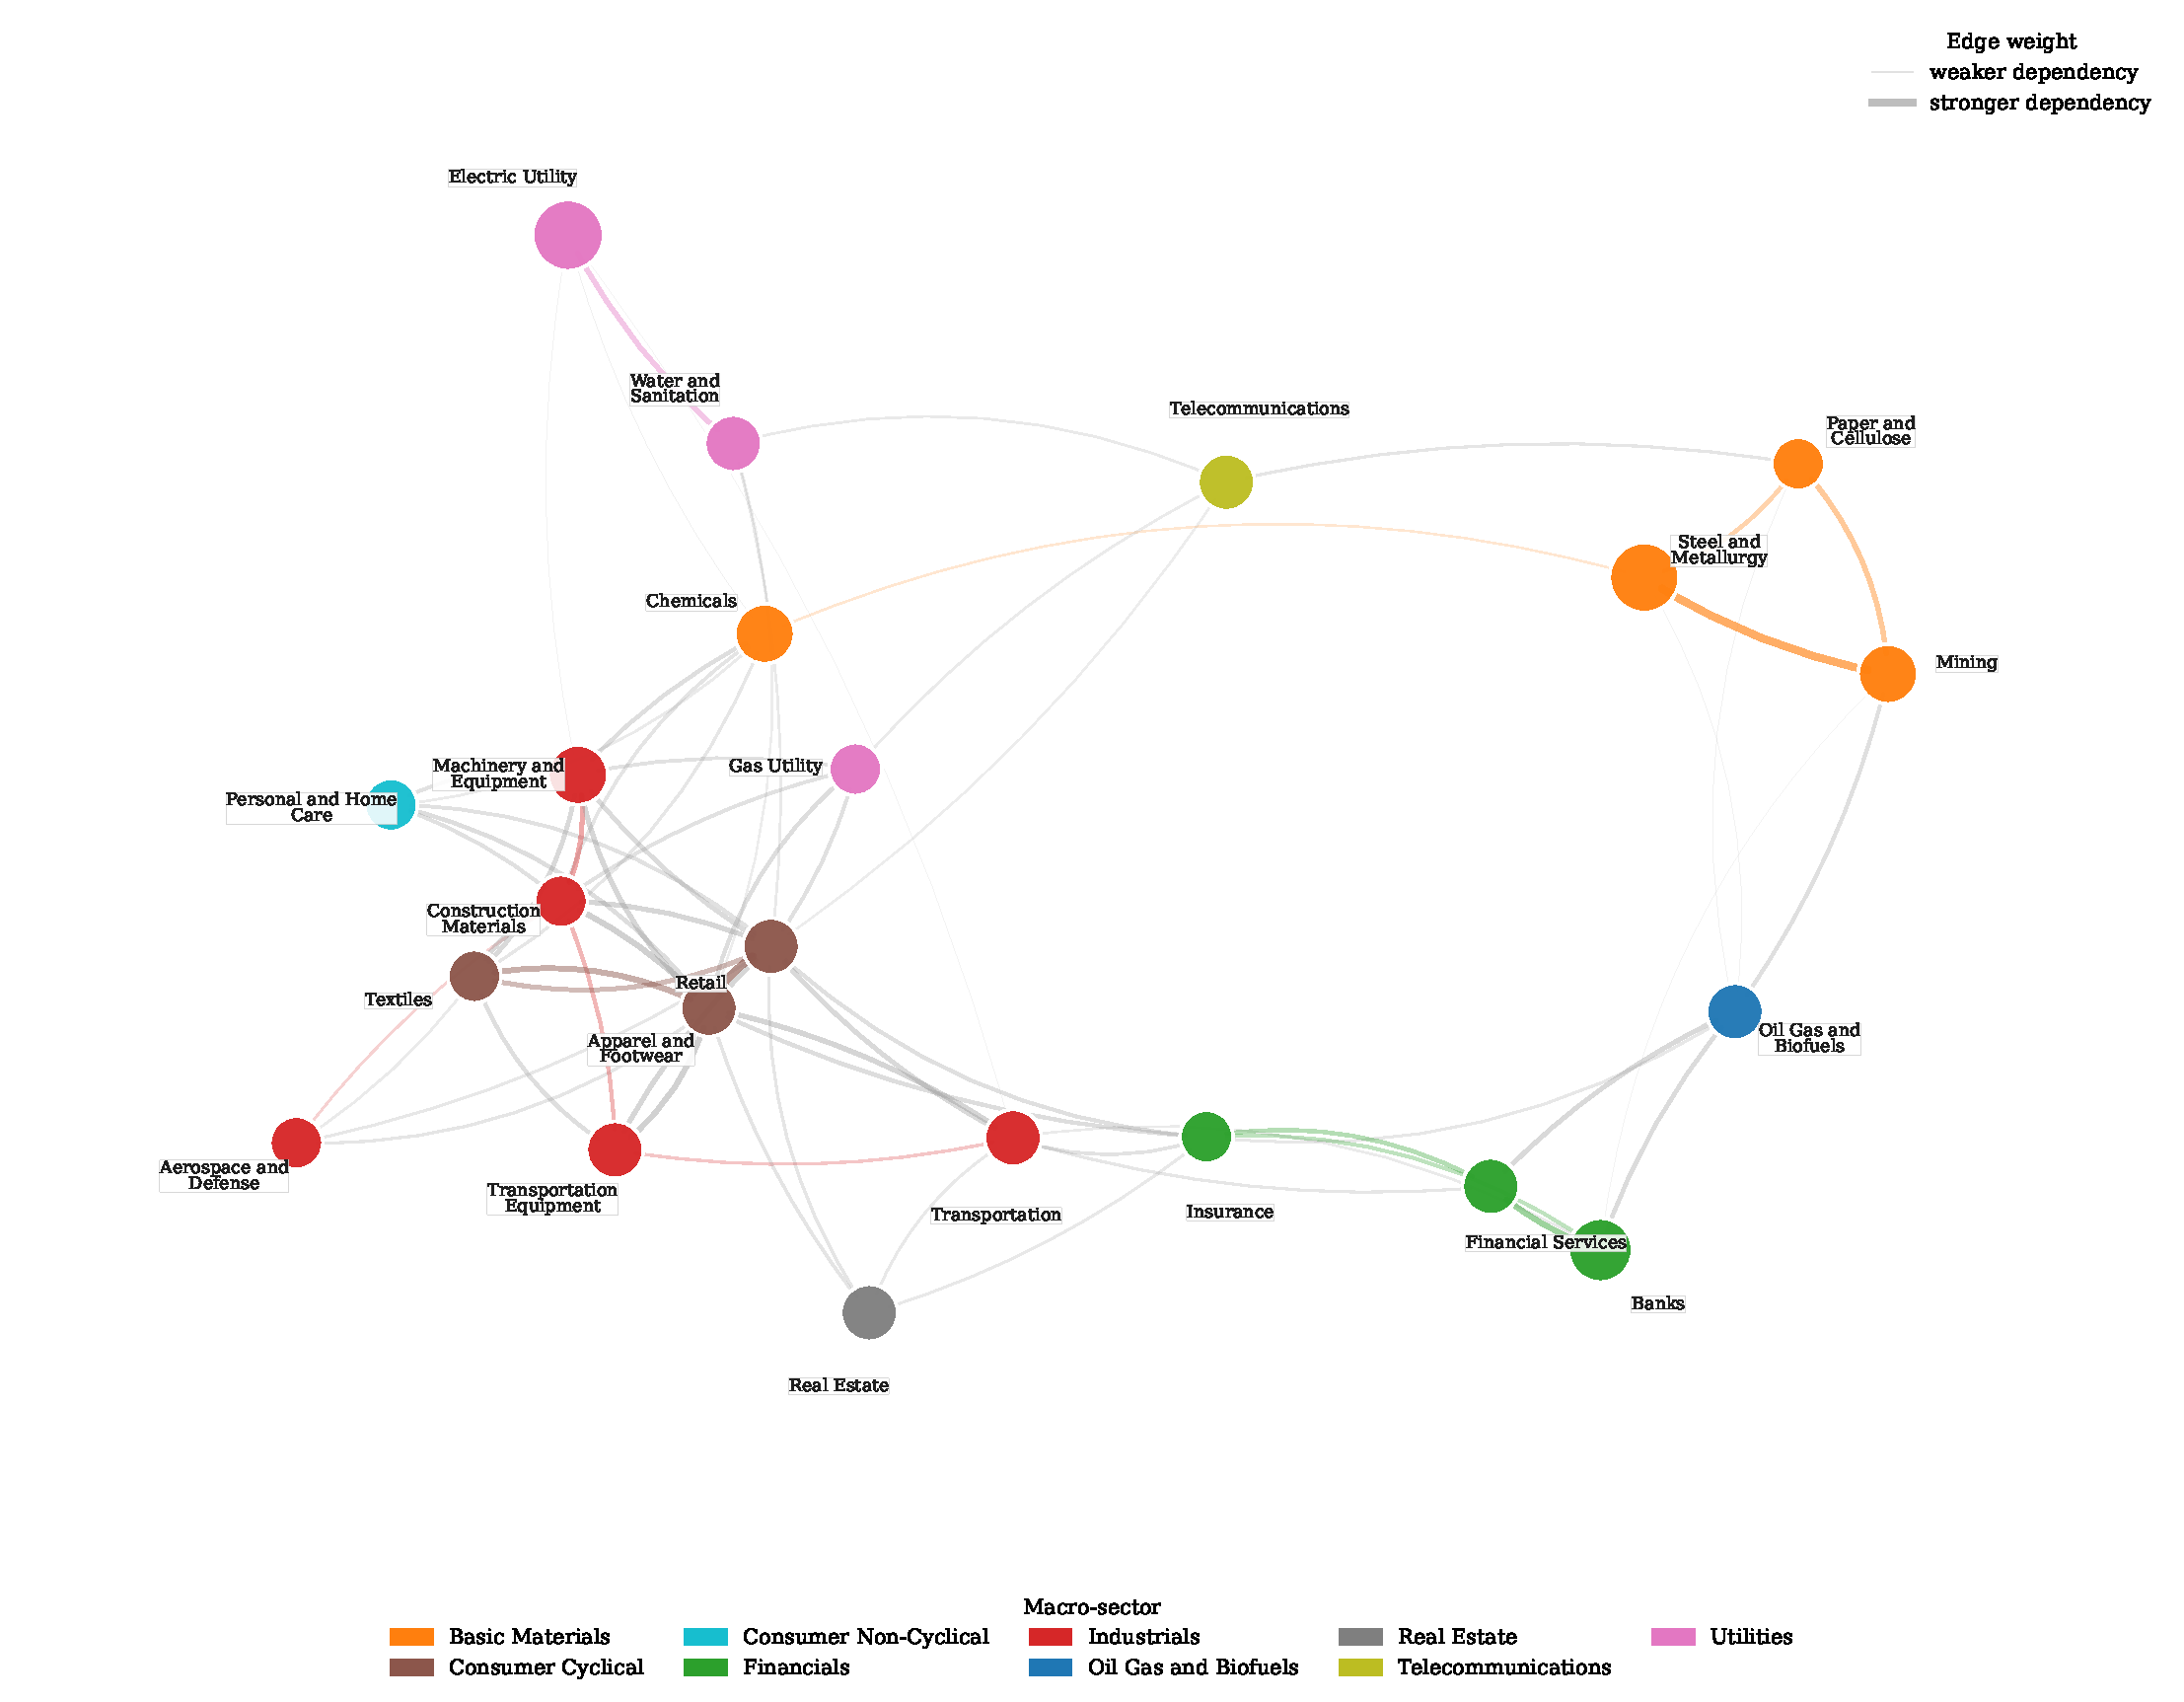
\includegraphics[
  width=0.92\linewidth,
  height=0.58\textheight,
  keepaspectratio
]{images/figure_15_subsector_dependency_network.pdf}
\captionof{figure}{Aggregated subsector dependency network. Nodes represent subsectors, node colour identifies the macro-sector and node size is proportional to the number of assets in the subsector. Edges represent retained subsector-level dependency weights, with thicker edges indicating stronger average dependency.}
\label{fig:subsector_network}
\end{center}
